\documentclass[a4paper]{article}
\usepackage[T1]{fontenc}
\usepackage[english]{babel}
\usepackage[utf8]{inputenc}
\usepackage[margin=3cm]{geometry}
\usepackage{longtable}
\usepackage{booktabs}
\usepackage{xcolor, colortbl}
\definecolor{headergray}{gray}{0.9} % Light gray for table headers
% \usepackage{amsmath}
% \usepackage{amssymb}
\usepackage{parskip}
% \usepackage{csquotes}
% \usepackage[hyperref,backend=biber,style=ieee,isbn=true,urldate=iso8601]{biblatex}
\usepackage[colorlinks=true, allcolors=blue]{hyperref}
% \usepackage{listings}
\usepackage{float}
\usepackage{graphicx}
\usepackage{caption}
\usepackage{mdframed}
\usepackage{array}

%% Hyperref options
\makeatletter
\hypersetup{
    linktoc=all,
    unicode=true,
    pdfcreator=,
    pdftitle={\@title},
    pdfauthor={\@author},
    pdfdisplaydoctitle=true,
}

\title{System Requirements}
\author{Jonathan Ahlström \and Ossian Gewert \and Jacob Jönsson \and Simon Persson \and André Roxhage \and Felix Sundholm}

\begin{document}
\maketitle

\begin{center}
    ETSN15 Requirements Engineering

Group Gamma

Jonathan Ahlström
Ossian Gewert
Jacob Jönsson
Simon Persson
André Roxhage
Felix Sundholm
\end{center}

\newpage
\tableofcontents
\newpage

\section{Introduction}
\subsection{Naming convention}
The naming convention used for requirements are descriptive camelCase names for Functional, Quality and Data requirements.

\subsection{Context Diagram}
The context diagram (\autoref{fig:context-diagram}) illustrates the systems key stakeholders in the inner domain. This includes travellers, travel agencies, airlines, IT maintenance and ad providers. In the outer domain, the context diagram shows marketing platforms, Google Maps for displaying maps and advertisers.
% André can update this if needed
% Explanation of diagram and its components
\begin{figure}[H]
    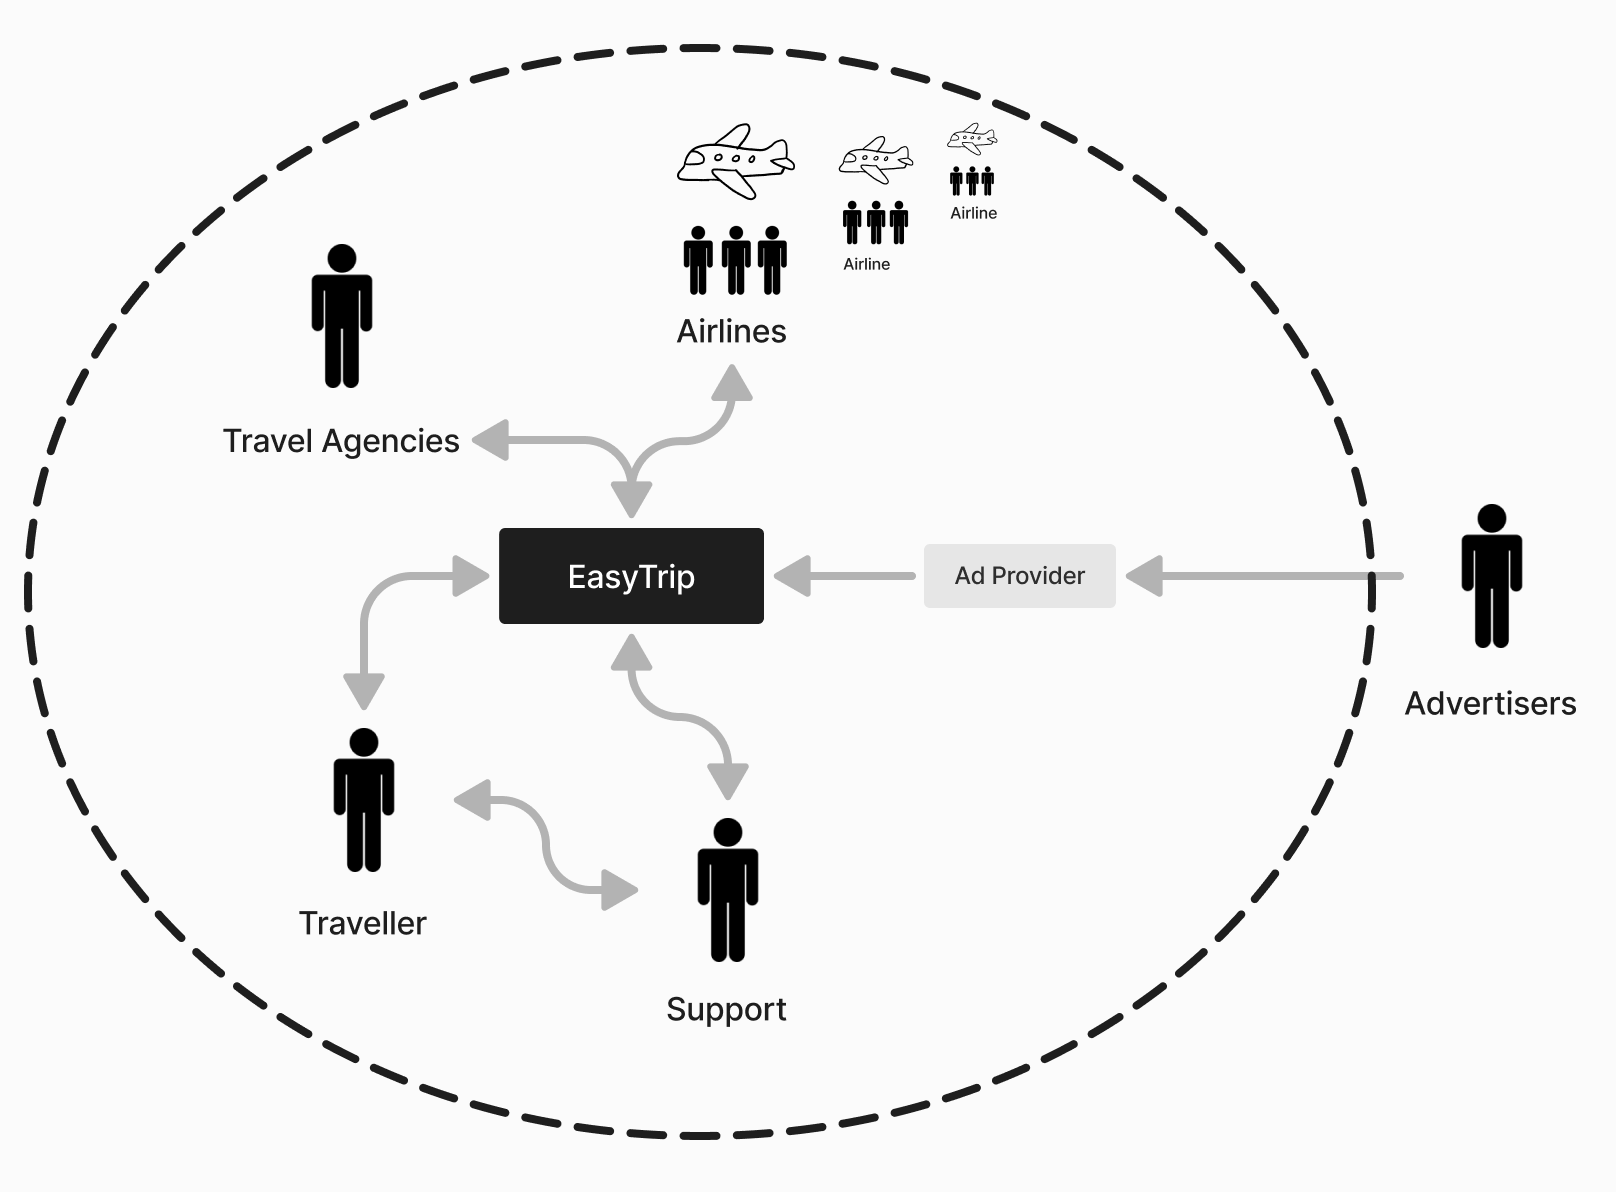
\includegraphics[width=.99\textwidth]{resources/contextDiagram.png}
    \caption{Context diagram}
    \label{fig:context-diagram}
\end{figure}

\subsection{Business Goals}
The system should help gain revenue by providing features that attract more customers and encourage existing customers to fly more. By differentiating the product from competitors, using unique data visualization, the system will gain a competitive advantage.
See \autoref{fig:mockup1} and \autoref{fig:mockup2} for a visual representation of the system.

The system should include features that improve customer satisfaction and loyalty, leading to _\% higher customer retention rates. This can be measured by customer satisfaction surveys, customer feedback and monitoring usage patterns.

The system should support features that enable the business to reach new markets and customer segments. This could include new types of users that not only want to find cheap flights, but also finds where they can travel for a certain budget.


\section{Elicitation}
% Jonathan & André
% Describe the elicitation process, what went well, what could have been done better. Interview, 1-2 persons, interview guide, semistructural interview. Then summarize the results in the elixitaion.tex.
\subsection{Elicitation of potential travellers}
In order to determine traveller goals and needs as well as to validate the product idea of Easytrip, we have elicitatied data from potential travellers. The data was collected from semistructured interviews with 2 participants. The particiapnts were chosen based on people that we know are frequent travelers. The interviews were conducted in a casual setting, and the recorded data is anonymous.

A interview guide was used to ensure consistency among the interviews. The guide was structured in three parts: Introduction, experience with existing travel planning tools, questions regarding the process to finding cheap flight, as well as closing questions. 

\subsubsection{Results}
The particiapnts (N=2) had an average age of 24 years and both had experience with using travel planning tools. The participants had different preferences when it came to finding cheap flights. 
... to-do sammanfatta resultaten, sub sub sub section?💕

\subsection{Prototype feedback}
Purpose: Test and validate an inital design of the system, to gather feedback on the traveller interface and functionality.

\subsection{Stakeholder Analysis}
Our stakeholders include competitors such as Momondo and Flight Scanner, travel agencies providing data partnerships, airline companies indirectly benefiting from bookings, end travellers, travelers, providing feedback, IT maintenance and development teams, and non-obvious actors such as the support department. Each stakeholder have different needs and goals, and it is important to understand these in order to create a successful product as well as to manage the relationships and expectations of the stakeholders.

\subsubsection{Airlines}
\subsubsubsection{Information Needed}
Since airlines are EasyTrips main source of data, information is needed regarding API endpoints for fetching price, date and times, availability based on travellers' search queries. Also, agreements on business models for affiliate links will be needed to ensure revenue channels. Additionally, real-time updates on flight status and any changes in schedules will be required to maintain accurate and up-to-date information for our travellers.

\subsubsubsection{Stake in the Platform}
Airlines benefit from increased visibility, effectively using EasyTrip as a marketing and sales channel. By providing accurate and real-time data, airlines can attract more customers and increase their revenue through the platform. The competition between airlines is also reflected in the platform, as travellers will compare prices and services, increasing the pressure on airlines to provide competitive offers and maintain high service quality.

\subsubsubsection{Risks}   
The platform has a strong dependency on airlines for providing accurate and timely data. Inconsistent or outdated flight information could negatively impact traveller experience and trust in our platform. Changes in airlines' API or business models could lead to disruptions and additional development costs and maintainment costs on our end. Airlines could withdraw from agreements, affecting our affiliate revenue stream. Any inaccuracies or delays in data could reflect poorly on their services and reputation.

\subsubsubsection{Solutions and Resources}
Airlines may suggest improvements such as dynamic pricing or marketing campaigns to maximize mutual benefits. Potential collaboration could be prioritizing a airline in the search results, or offering exclusive deals to travellers. These collaborations could be beneficial for both parties, as it would increase the visibility of the airline and create a new revenue stream for us.

\subsubsection{Travel Agencies}
\subsubsubsection{Information Needed}
Travel agencies provide data partnerships and EasyTrip needs access to their data regarding flight offers in a similar way that we are dependent on the airlines' data.

\subsubsubsection{Stake in the Platform}
Travel agencies benefit by reaching more customers through the platform in a similar way as for airlines. The main difference is the advantage of being able to combine multiple airline in routes including multiple layoveers. This is a service that airlines do not provide. Therefor, travel agencies can promote deals and lead customers to additional purchases since they also provide accomodations and other travel services. Both airline and travel agencies benefit from increased visibility and bookings through the platform, effectively using us as a marketing and sales channel.

\subsubsubsection{Risks}
There are risks that travel agencies could provide inconsistent data, leading to inaccurate package pricing or availability issues. Competition between agencies could result in disputes over featured listings. Also, there is a risk of agencies withdrawing from agreements, affecting our affiliate revenue stream. The platform is dependent on the travel agencies for providing accurate and timely data. Similar to the airline can changes to API or business models could lead to disruptions and additional development costs and maintainment costs on our end. Favoring of competitors could also be a risk, as the agencies might prioritize other platforms over EasyTrip. The agencies might have exclusive deals and partnerships with other platforms, which could limit the provided data.

\subsubsubsection{Solutions and Resources}
Similar to the airlines is the potential to include promotional campaigns targeting high-demand destinations. This could be beneficial for both parties. However, such aggreement would need to be carefully negotiated to ensure that both parties benefit from the collaboration, without hurting the relationship to other stakeholders. For the development process, travel agencies could also provide feedback on the platform and suggest improvements to the traveller interface or features to ensure that their data is presented in the best possible way.

\subsubsection{Travellers}
\subsubsubsection{Information Needed}
To provide a personalized experience, the platform needs information about travellers budget constraints, destinations and travel dates. Optionally, personal data such as email can be gathered to enable notifications on price changes. Also, feedback on their traveller experience crucial for the improvement and future of EasyTrip.

\subsubsubsection{Stake in the Platform}
travellers benefit from accurate, real-time price comparisons, and personalized recommendations. They gain time efficiency and cost savings when planning trips. Additionally, travellers are the main source of revenue for the platform, as they generate bookings and affiliate revenue. Therefore, user satisfaction and loyalty are crucial for the success of the platform. By providing feedback and suggestions, travellers can influence the platform's development and improve their overall experience. This could lead to increased retention and engagement, meaning travellers will return to the platform for future travel planning.

\subsubsubsection{Risks}
The dependency on airlines is a factor that can generate issues such as inaccurate flight information, delayed notifications, or privacy concerns. If travellers feel their data is not secure or their preferences are not being met, they may lose trust in the platform and seek alternatives.

\subsubsubsection{Solution och Resources}
To mitigate these risks, EasyTrip will implement validation and consistency checks to ensure accurate flight information. Additionally, the platform will provide clear and transparent privacy policies to address any privacy concerns. Regular traveller feedback will also be gathered by interviews and forums to identify possible problems with the system. 

\subsubsection{IT Support and Maintenance}
\subsubsubsection{Information Needed}
The IT support team requires a comprehensive administration interface to monitor system errors, API updates, and data quality from airlines and travel agencies. They need access to logs, error reports, and real-time data feeds to ensure the system's integrity and performance. Since payment and booking are handled by airlines or travel agencies, the IT support team does not need access to payment information, allowing them to focus on technical issues and system maintenance.

\subsubsubsection{Stake in the Platform}
The IT support team is crucial for maintaining the platform's reliability and performance. They ensure that data from airlines and travel agencies is accurate and up-to-date, which is essential for traveller trust and satisfaction. By resolving technical issues promptly and ensuring seamless API integrations, the IT support team helps maintain the platform's reputation and operational efficiency.

\subsubsubsection{Risks}
The IT support team faces risks such as system downtime, and technical issues that could disrupt the platform's functionality. Not enough monitoring and delayed response to issues can lead to prolonged outages, negatively impacting traveller experience and trust. Additionally, the team must stay updated with API changes from airlines and travel agencies to prevent integration issues. To resolve this, a error handling system must be in place to detect and address issues promptly.

\subsubsubsection{Solutions and Resources}
To mitigate these risks, the IT support team will implement robust monitoring and alerting systems to detect and address issues promptly. Regular updates and maintenance schedules will be established to ensure system stability. Collaboration with airlines and travel agencies will be maintained to stay informed about API changes and updates. Additionally, the team will conduct regular data quality checks and validation processes to ensure the accuracy and reliability of the information presented on the platform.

\subsubsection{Competitors - Momondo, Flight Scanner - TOOO DOOO 💩}
\subsubsubsection{Information Needed}
Write this!!! Using the bullet poitnts isch 🤓
\begin{itemize}
    \item \textbf{User Experience Feedback:} Gather reviews and feedback from users of competitor platforms to identify common pain points and areas for improvement.
    \item \textbf{Feature Comparison:} Compare the features offered by competitors, such as search filters, booking options, and user interface design, to identify gaps and opportunities for innovation.
    \item \textbf{Pricing Models:} Understand the pricing strategies and commission structures of competitors to ensure competitive pricing and better deals for travellers.
    \item \textbf{Market Positioning:} Analyze how competitors position themselves in the market, including their marketing strategies and target demographics, to identify potential niches or underserved segments.
    \item \textbf{Technical Performance:} Evaluate the technical performance of competitor platforms, including website speed, mobile app functionality, and API reliability, to ensure EasyTrip offers a superior technical experience.
    \item \textbf{Customer Support:} Assess the quality and availability of customer support provided by competitors to identify areas where EasyTrip can offer better service.
\end{itemize}

\subsubsubsection{Stake in the Platform}
Simularly to EasyTrip, competitors benefit from increased visibility and bookings through their platform. 

\subsubsubsection{Risks}
Competitors are heavily reliant on the flight industry, as their services would not generate any income if there were no active flights. Their business model and traveller base are directly tied to the demand for air travel.


\subsubsubsection{Solutions and Resources}
Competitors have an established role in the industry, providing travellers with alternative platforms for flight comparisons and bookings. 

\subsection{Conflicting Stakeholder Interests}
Make a table with conflicting interests and how to solve them

Write a paragrapgh about how to solve them and the stakeholders relationship to each other


\newpage
\section{Requirements Specification}
The requirements in this document follow a hierarchical structure where indented requirements represent data or quality requirements that are connected to their parent functional requirement. This structure helps show the relationships between functional requirements and their associated quality attributes or data specifications.

For example, a functional requirement like \textbf{HeatmapSearch} may have indented quality requirements such as \textbf{HeatmapPerformance} that specify performance criteria for that feature.

\subsection{Heatmap Visualization}

\begin{tabular}{|p{.95\textwidth}|}
    \hline
    \textbf{Task:  Find cheap trip destination using heatmap}\\
    \hline
    Subtasks:
    \begin{enumerate}
        \item Input origin / allow location data
        \item Input flight dates
        \item Navigate heatmap
        \item Select area
        \item Select show details for flight
        \item Get referred to airline
    \end{enumerate}\\
    \hline
    Variants:
    \begin{enumerate}
        \item[1a.] User types in origin airport
        \item[1b.] User uses device location data for origin
    \end{enumerate}\\
    \hline
\end{tabular}

\textbf{HeatmapSearch}: The system shall display a heatmap that visually represents flight prices for various destinations, with the lowest available prices highlighted using colors, engaging users in the search process. See an example in \autoref{fig:mockup2}.
    \begin{quote}
        \textbf{HeatmapPerformance}: The heatmap should update dynamically within 3 seconds of data input or changes such as price range. \\ \\
        Monitor UI logs to confirm rendering completion time after changes to input data.
    \end{quote}
    \begin{quote}
        \textbf{HeatmapVisibility}: The heatmap shall be responsive and maintain readability on screen sizes ranging from 320px (mobile) to 1920px (desktop). It shall use a color gradient that ensures a minimum contrast ratio of 4.5:1 (WCAG AA) for text labels and distinguishable color differences between price categories. See \autoref{fig:mockup1} and \autoref{fig:mockup2}. Note the examples are only prototypes and are not final.
    \end{quote}
\textbf{DateRangeMap}: Travellers and Travel Agencies can change the dates for which the map shows data. Domain-level control for flight search customization.
    \begin{quote}
        \textbf{DateChangeResults}: The map should reflect date changes in under 2 seconds without requiring a full reload. \\ \\
        Monitor UI logs to confirm rendering completion time after date modifications.
    \end{quote}
\begin{quote}
    \textbf{FlexibleRangeMap}: The system should support flexible date ranges spanning at least 30 days for price comparisons. \\ \\
    Test by selecting a range of 30-60 days, verifying the system returns results across all days without errors.
\end{quote}
\textbf{ListFlightsFromMap}: Travellers and Travel Agencies can see a text list of destinations with the lowest flight prices shown on map. Product-level display of destinations based on search.
    \begin{quote}
        \textbf{TextListsShown}:Destination lists should be updated in real-time when new flight deals become available. \\ \\
        Insert a new deal in the back-end or get deal from airlines API and verify update propagation within milliseconds.
    \end{quote}
\textbf{AirportSelection}: Travellers and Travel Agencies can select airports from the heatmap. Product-level feature allowing interactive selection.
\begin{quote}
    \textbf{FastAirportSelection}: Selected airports should be highlighted instantly and search results updated in under 2 seconds. \\ \\ 
    Measure UI update times via browser dev tools or performance logs.
\end{quote}

\subsection{User Security}
\textbf{LawCompliance}:The system should comply with general data protection regulations (GDPR). Domain-level requirement ensuring user data privacy.
\begin{quote}
    \textbf{GDPRCompliance}: Perform a data protection regulations (GDPR) audit to ensure compliance with data protection regulations. \\ \\
    Document and address any issues found during the audit.
\end{quote}
\textbf{SecureDataEncryption}: User data should be encrypted both in transit and at rest. Domain-level security requirement.
\begin{quote}
    \textbf{DataEncryptionCheck}: Ensure that all user data is encrypted using secure protocols and stored securely. \\ \\
    Perform security audits and penetration tests to verify encryption and storage mechanisms.
\end{quote}

\subsection{Flight Search}

\begin{tabular}{|p{.95\textwidth}|}
    \hline
    \textbf{Task: Find cheap flight}\\
    \hline
    Purpose: Find cheap flight to general area\\
    \hline
    Input parameters:
    \begin{itemize}
        \item Origin
        \item Destination
        \item Dates
    \end{itemize}\\
    \hline
    Display options:
    \begin{itemize}
        \item Heatmap
        \item List
        \item Filter
        \item Date sliders
    \end{itemize}\\
    \hline
\end{tabular}

\textbf{SearchCheapFlights}: Travellers and Travel Agencies can find destinations with low flight prices when providing a departure city and dates. Search results shall be ranked by price in ascending order, ensuring the most cost-effective options are prominently displayed. Goal-level requirement defining a key system function.
\begin{quote}
    \textbf{FastSearchResults}: Search results should be displayed within 2 seconds for queries that include a departure city, and travel dates, retrieving data for up to \_ available flights.\\ \\ 
    Tested by generating random inputs and measuring response time using automated performance testing tools, logging response times for 1000+ random queries.
\end{quote}
\textbf{ListCheapFlights}: The system shall present a structured list of available flights to a specified destination, sorted by price in ascending order. Product-level feature for displaying search results.
\begin{quote}
    \textbf{TextListSupport}: The list should support sorting by price, duration, and airline, with sorting applied in under 1 second.\\ \\ 
    Use UI performance tests to time sorting actions on datasets of varying sizes for example destinations with a lot of flights or destinations with less flights.
\end{quote}
\textbf{SearchCheapDestinations}: Travellers and Travel Agencies can find flights to a given destination. Domain requirement focusing on the flight search feature.
\begin{quote}
    \textbf{FastPriceDisplay}: The system shall retrieve and display flight prices within 2 seconds for search requests that include a departure city, and travel dates, processing up to \_ flight options per request.\\ \\
    Execute automated tests simulating 1000+ searches and log the response time until results are fully rendered. Primarily same as \textit{FastSearchResults}.
\end{quote}
\textbf{DateRangeSearch}: Travellers and Travel Agencies should be able to provide a range of possible dates for their flight search making the service more flexible and appealing to a wider range of users. Domain-level functionality supporting flexible searches, in flight search feature.
\begin{quote}
    \textbf{DateRangeCheck}: The system should support flexible date ranges spanning at least 30 days for price comparisons. \\ \\
    Test by selecting a range of 30-60 days, verifying the system returns results across all days without errors.
\end{quote}
\textbf{GeolocationService}: Travellers can have their device provide their current location. Domain-level feature leveraging geolocation services.
\begin{quote}
    \textbf{GeoLocationCheck}:Location detection should be completed in under 3 seconds with at least 95\% accuracy.\\ \\
    Use GPS data from 50 ore more test cases across different devices and measure accuracy based on expected vs. detected locations.
\end{quote}
\textbf{ShowFlights}: Traveller can click through to ticket booking page for shown flights. Product-level requirement enabling ticket purchase.
    \begin{quote}
        \textbf{CorrectNavigation}: Clicking a flight should navigate to the booking page within 1 second and fill in relevant details from users account. \\ \\
        Use automated UI testing to time redirection and fill in data according to users account.
    \end{quote}
\textbf{SaveFavoriteCity}:A signed-in traveller can save favorite cities. Product-level feature for personalization.
\begin{quote}
    \textbf{FavoriteCityFetching}: Favorite cities should be stored in under 5 seconds and retrievable in under 1 second. \\ \\
    Save favorite cities and time retrieval speed via API performance monitoring.
\end{quote}

\subsection{User Experience}
\textbf{UsabilityScore}: The ease of use of the product shall be tested and must achieve a System Usability Score (SUS) of at least 70 points, indicating acceptable usability.
\begin{quote}
    \textbf{SUSTesting}: Conduct usability tests with a sample group of users and calculate the SUS score. \\ \\
    Ensure the average score meets or exceeds 70 points.
\end{quote}

\textbf{AccessibilityCompliance}: The accessibility of the product shall be tested and must comply with WCAG 2.1 standards.
\begin{quote}
    \textbf{WCAGTesting}: Perform accessibility audits using automated tools and manual testing to ensure compliance with WCAG 2.1 standards. \\ \\
    Document and address any issues found during testing.
\end{quote}

\textbf{RegularUserFeedback}: The system shall regularly prompt users for feedback. Product-level feature that aims to gather user insights and improve customer satisfaction by understanding user experiences and expectations. 
\begin{quote}
    \textbf{FeedbackCheck}: After \_ hours of use, the system shall prompt the user with the question "What do you think about EasyTrip?" and a rating scale. 
\end{quote}

\subsection{Account Management \& Personalization}
\textbf{AccountCreation}: Travellers should be able to create accounts. Product-level requirement for account management.
\begin{quote}
    \textbf{AccountData - Data dictionary}: Product-level requirement: \\\textbf{Class}: User\\
    The user is a Traveller or Travel Agency who has a user account in the product.
    
    \textbf{Examples}:
    1. A traveller who has a user account.
    2. A travel agency who uses their user account to search flights.
    
    \textbf{Attributes}:
    \begin{enumerate}
        \item \textbf{email}:      Text, 320 chars
        The user's email address. This email address is used for communication with the user outside the product.
        \item \textbf{name}:       Text, 50 chars
                The name of the traveller or travel agency using the account.
        \item \textbf{newsletter}: Boolean
        Whether the user wants mass email's from the product or not.
        \item \textbf{city}:       Text, 35 chars
        The city the user's default origin is set to. This is the standard origin used when performing searches for the user.
    \end{enumerate}    
\end{quote}

\begin{quote}
    \textbf{AccountData - Virtual window}: Product-level requirement described using a data dictionary: \\\textbf{Class}: \begin{longtable}{|p{3cm}|p{9cm}|}
        \hline
        \rowcolor{headergray}
        \textbf{Field} & \textbf{Value} \\ \hline
        \textbf{Email} & exampleJohn@gmail.com \\ \hline
        \textbf{Name} & John Doe \\ \hline
        \textbf{Utskick} & True \hspace{1em} False \\ \hline
        \textbf{City} & New York \\ \hline
    \end{longtable}
\end{quote}

\textbf{EmailConfirmation}: The ownership of travellers' email addresses should be confirmed. Domain requirement ensuring valid accounts.
    \begin{quote}
        \textbf{ConfirmationCheck}: Email verification links should be sent within 5 seconds and expire after 24 hours. \\ \\
        Log email dispatch times in the system and verify expiration behavior after 24 hours.
    \end{quote}
\textbf{CreateAccountEmail}: Travellers should be able to create accounts with email addresses and passwords. Productlevel authentication requirement.  
    \begin{quote}
        \textbf{}: The registration process should take no longer than 15 seconds, including email verification. \\ \\
        Automate user sign-ups and measure time from form submission to receiving the verification email.
    \end{quote}
\textbf{EmailChange}: Travellers should be able to change their email address. Product-level account management feature.
\begin{quote}
    \textbf{EmailChangeConfirmationPerformance}: Changes to email addresses should be confirmed within 10 seconds via a verification email.\\ \\
    Track the end-to-end time from submission of email change request to email receipt.
\end{quote}
\textbf{ChangePassword}:Travellers should be able to change their passwords. Product-level security feature.
    \begin{quote}
        \textbf{CheckChangePassword}:Password changes should be effective after 5 seconds and require strong passwords (at least 8 characters, uppercase, lowercase, number, symbol). \\ \\
        Verify enforcement of password complexity rules and Ensure old credentials become invalid 5 seconds after post-update.
    \end{quote}
\textbf{PasswordReset}: Travellers should be able to reset their password if they have forgotten it. Product-level usability requirement.
\begin{quote}
    \textbf{FastPasswordReset}: Reset emails should be sent within 10 seconds and expire after 30 minutes. \\ \\
    Log email dispatch times and attempt password resets after 30 minutes to confirm expiration.
\end{quote}
\textbf{MarketingConsent}: Travellers should be asked about receiving marketing emails during account creation. This consent should be editable in real-time in the Account management section. The system should log consent preferences for auditing purposes. Domain-level requirement ensuring compliance with marketing preferences.
\begin{quote}
    \textbf{EmailPreferenceCheck}:Marketing email preferences should be configurable and updated in real-time. \\ \\ 
    Toggle marketing settings in the Account management section and verify backend logs reflect changes within 5 seconds.
\end{quote}

\subsection{System Performance}
\textbf{StatisticsReport}: Product manager can request a statistics report. Goal-level requirement for system analytics.
\begin{quote}
    \textbf{FastStatisticsReport}: Reports should be generated in under 10 seconds for a dataset covering the last 6 months. \\ \\
    Execute test report requests and measure query execution and rendering time.
\end{quote}
\textbf{AnonymizedData}: User data should be anonymized for analytics. 
\begin{quote}
    \textbf{AnonymizedCheck}: Ensure that all personally identifiable information (PII) is removed or obfuscated before generating reports. Verify through data audits and compliance checks. \\ \\
\end{quote}
\textbf{DynamicResourceAllocation}: The system should allocate computing resources (for example memory and CPU), dynamically based on load to ensure scalability. Goal-level requirement for system scalability.
\begin{quote}
    \textbf{ResourceAllocationCheck}: The system should scale up to handle _ concurrent users without slowdown. \\ \\
    Simulate _concurrent users with load-testing tools and measure system response time. For example AWS.
\end{quote}
\textbf{UptimeGuarantee}: The system should have an uptime of at least 99.9\%. Goal-level requirement for system reliability.
\begin{quote}
    \textbf{UptimeMonitoring}: Monitor system uptime and ensure it meets the 99.9\% requirement. \\ \\
    Use uptime monitoring tools to track system availability over time.
\end{quote}
\textbf{AutoFailoverMechanism}: The system should have an automatic failover mechanism. The system should automatically switch to a backup server in case of a failure. Goal-level requirement for system reliability.
\begin{quote}
    \textbf{FailoverTesting}: Simulate a system failure and verify that the failover mechanism is triggered within 5 seconds. \\ \\
    Use automated tests to simulate system failures and measure failover time.
\end{quote}
\textbf{APIIntegrationSupport}: The system should support integration with external APIs. Goal-level requirement for system extensibility.
\begin{quote}
    \textbf{APIIntegrationCheck}: Ensure that the system can integrate with at least the necessary external APIs without performance degradation. \\ \\
    Test system performance with and without API integrations to measure impact.
\end{quote}

\subsubsection{Data Model}
\textbf{DataModel}: The product level data requirements are represented through a E/R diagram in \autoref{fig:data-model}, it shows the data used \\ \\
for the flight searches and the user accounts in the system.

\begin{figure}[H]
    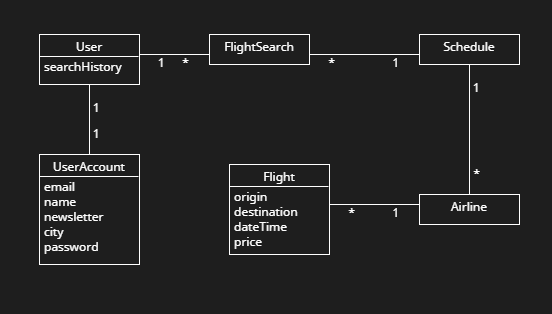
\includegraphics[width=1\textwidth]{resources/dataRelations.PNG}
    \caption{Entity/Relationship data model}
    \label{fig:data-model}
\end{figure}

\subsection{Others}
\textbf{MultipleTicketPrices}: Travellers and Travel Agencies can see prices for multiple tickets. Product-level requirement enabling comparison of ticket prices.
\begin{quote}
    \textbf{FastMultiTicketPrices}: The system should allow searching for up to 10 passengers simultaneously without affecting response time. Test by searching for 10 tickets and verifying that all prices are displayed without errors.\\ \\
     Compare response times of searches with 1 vs. 10 passengers under normal and peak loads.
\end{quote}
\textbf{MultiFlightTrips}: Travellers and Travel Agencies can find prices of multi-flight trips. Product-level requirement for multi-leg trip pricing.
    \begin{quote}
        \textbf{PriceRetrieval}:The system should retrieve multi-flight prices in less than 5 seconds, considering layovers and airlines. \\ \\ 
        Run tests for complex multi-leg searches, logging response times for different scenarios.
    \end{quote}
\textbf{MarketingChannels}: Marketers can send marketing emails to travelers who have explicitly opted in through the account management settings. Product-level marketing function.
\begin{quote}
    \textbf{CheckMarketing}: Marketing emails should be delivered to 95\% of recipients within 1 minute of sending. \\ \\
    Track email delivery timestamps for mass campaigns and compute success rate over time.
\end{quote}
\textbf{B2BFindFlights}: Travel agencies can find flights on behalf of clients. Goal-level requirement supporting B2B services.
\begin{quote}
    \textbf{B2BMultipleSearch}: Travel agency accounts should support handling at least 50 concurrent searches without slowdown. \\ \\ 
Simulate 50+ concurrent users with load-testing tools for example JMeter and measure system response time.
\end{quote}

%TODO ADD DESCRIPTION TO FOLLOWING PART
\begin{table}[h]
    \centering
    \renewcommand{\arraystretch}{1.5}
    \begin{tabular}{|l|c|c|c|c|c|}
        \hline
        & \textbf{Critical} & \textbf{Important} & \textbf{As usual} & \textbf{Unimportant} & \textbf{Ignore} \\
        \hline
        \textbf{Operation} & & & & & \\
        Integrity/security & & & x & & \\
        Correctness & & & x & & \\
        Reliability/availability & 1 & & & & \\
        Usability & 3 & & & & \\
        Efficiency & & 2 & & & \\
        \hline
        \textbf{Revision} & & & & & \\
        Maintainability & & & x & & \\
        Testability & & & x & & \\
        Flexibility & & & x & & \\
        \hline
        \textbf{Transition} & & & & & \\
        Portability & & & & x & \\
        Interoperability & & 4 & & 4 & \\
        Reusability & & & & & x \\
        Installability & & 5 & & & 5 \\
        \hline
    \end{tabular}
    \caption{Software Quality Characteristics}
    \label{tab:quality_characteristics}
\end{table}

\subsection*{Explanations}
\begin{enumerate}
    \item It is critical that the system is always available since it can be used by anyone across the world, meaning we have the potential to gain customers at any time of the day. If availability is below 99\%, the company loses money, and key stakeholders, such as airlines, are negatively impacted.
    \item If the system cannot filter or return proper search results quickly, users may grow impatient and leave for a competitor.
    \item The system must be easy to navigate and use since our customer base includes anyone willing to travel. Users will have a wide range of experience using websites. \textbf{TODO:} Our differentiation lies in ease of learning and user satisfaction with how we display data.
    \item The system is not required to interact with other systems like file transfers or specific hardware. However, some components need to cooperate with external systems, such as our ad provider or direct links to airlines for flight booking.
    \item Since the system is web-based on computer workstations, installation is unnecessary. However, for the mobile version, an app must be installed, which should be easy to download from platforms like the App Store or Google Play.
\end{enumerate}

\newpage
\begin{figure}[h]
    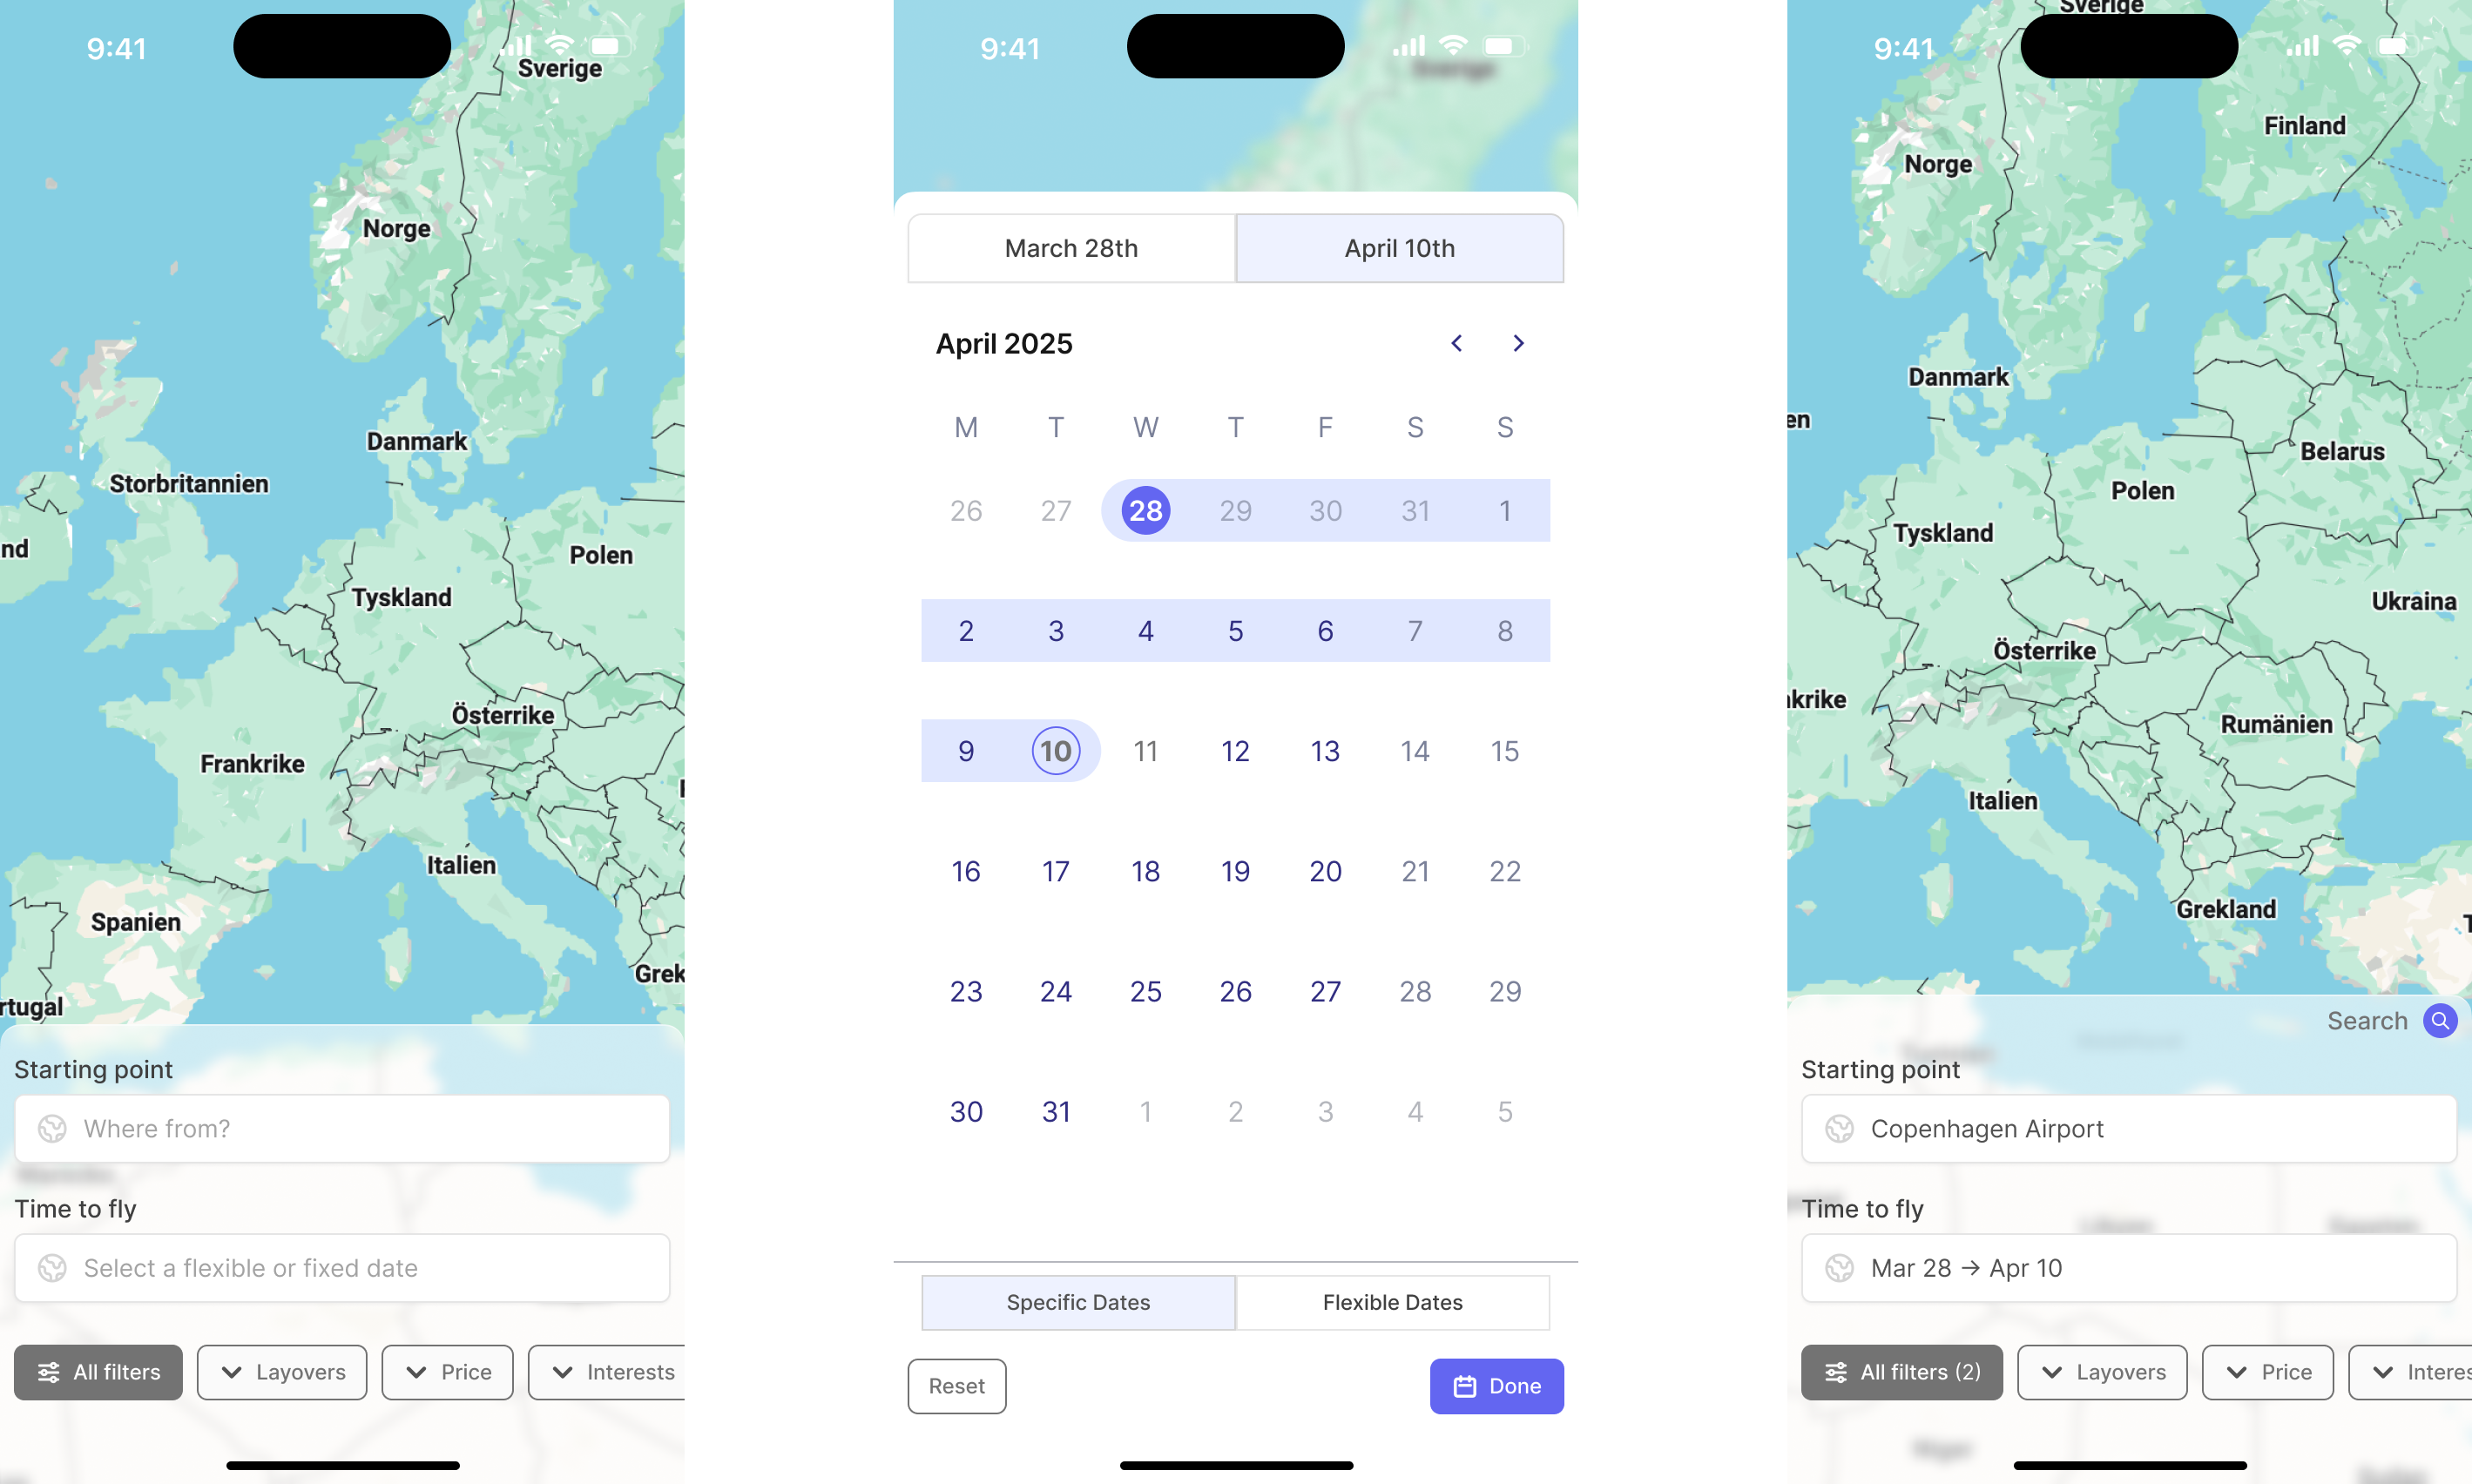
\includegraphics[width=.89\textwidth]{resources/mockup1.png}
    \caption{User interface showing the search page, dynamic date picker and filters.}
    \label{fig:mockup1}
\end{figure}

\begin{figure}[h]
    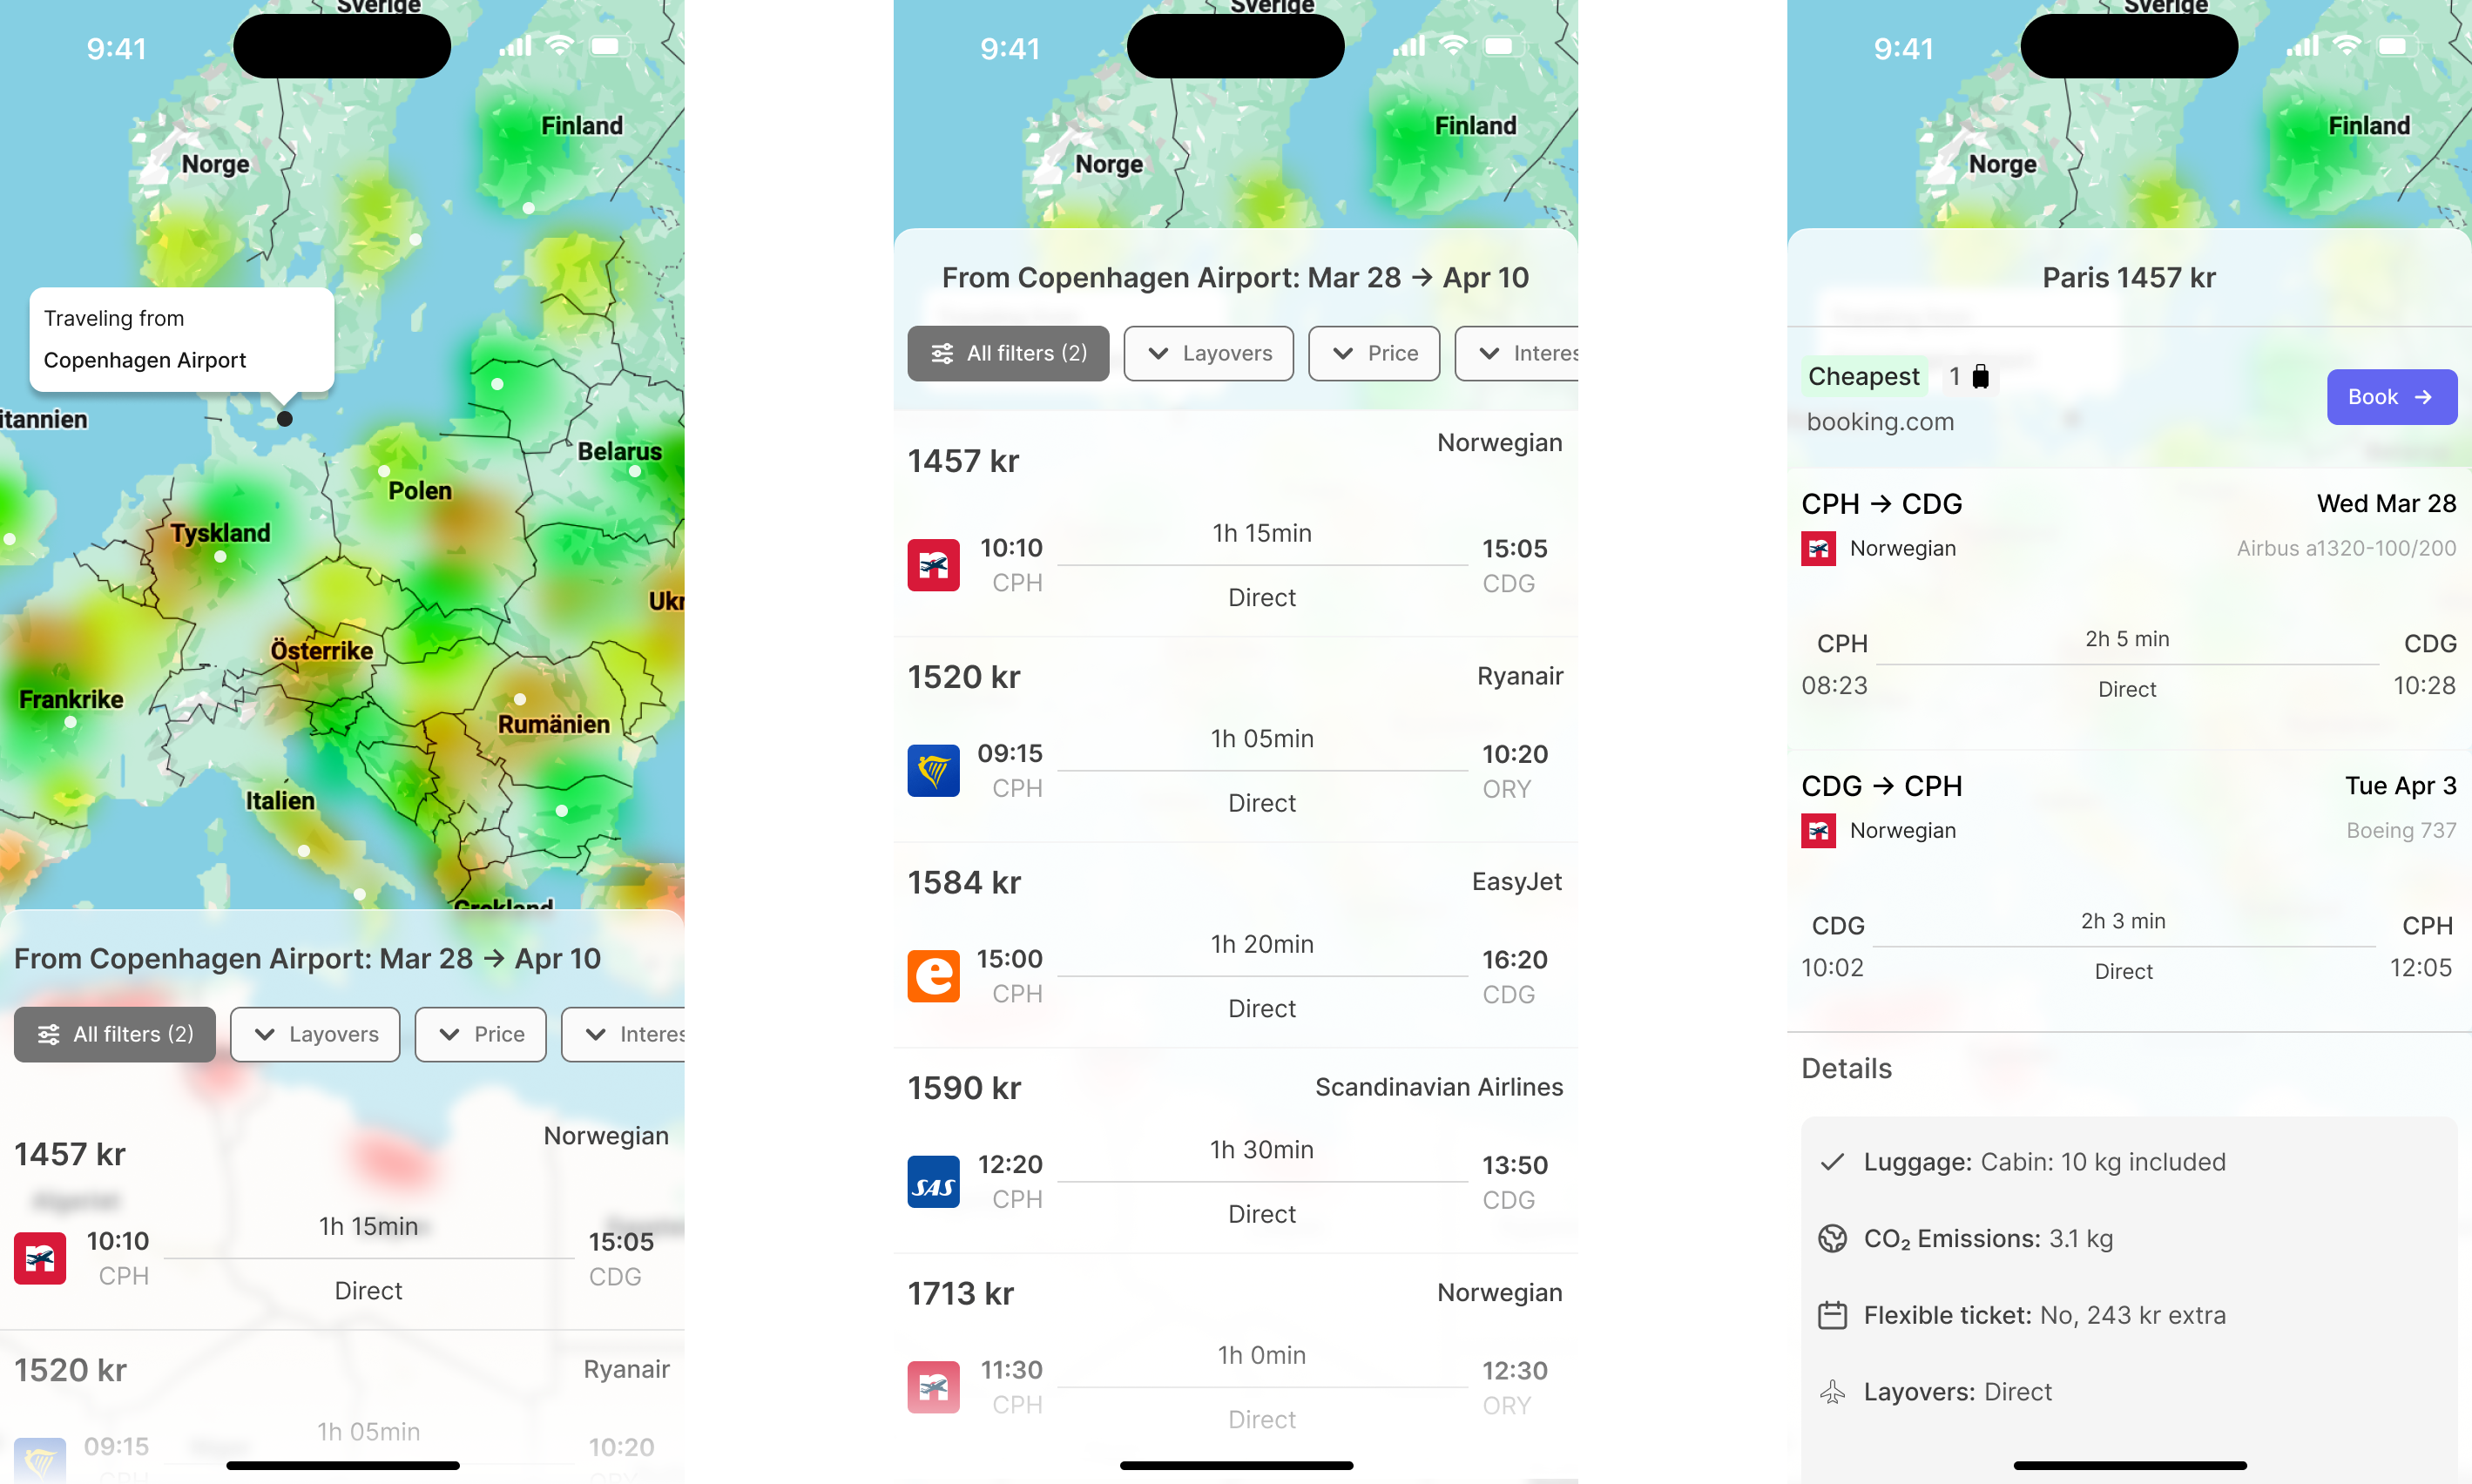
\includegraphics[width=.89\textwidth]{resources/mockup2.png}
    \caption{User interface showing the search results page with a list of flights and a heatmap.}
    \label{fig:mockup2}
\end{figure}

\newpage



\section{Release Plan \& Prioritization}
\begin{longtable}{|c|c|c|c|}
    \hline
\rowcolor{headergray}
\textbf{Release} & \textbf{Feature} & \textbf{Priority} & \textbf{Prioritization Motivation / Explanation} \\
\hline
\endfirsthead
\rowcolor{headergray}
\hline
\textbf{Release} & \textbf{Feature} & \textbf{Priority} & \textbf{Prioritization Motivation / Explanation} \\
\hline
\endhead
\hline
\endfoot
\hline
\endlastfoot

4 & Feature 1 & High & Explanation for Feature 1 \\
4 & Feature 2 & Medium & Explanation for Feature 2 \\
4 & Feature 3 & Low & Explanation for Feature 3 \\
\hline
5 & Feature 1 & High & Explanation for Feature 1 \\
5 & Feature 2 & Medium & Explanation for Feature 2 \\
5 & Feature 3 & Low & Explanation for Feature 3 \\
\hline

\end{longtable}

% \section{Functional Requirements}
% Ossian
% Describe what the system does, i.e., the services it provides to the users.
% % \subsection{Functional Requirements}
The following functional requirements have been identified for the EasyTrip system.

F1-G: Travellers can find destinations with cheap flights when providing a departure city and dates.
    Goal-level requirement defining a key system function.
    
F2-D: Travellers should be able to provide a range of possible dates.
    Domain-level functionality supporting flexible searches.
    
F3-D: Travellers can have their device provide their current location.
    Domain-level feature leveraging geolocation services.
    
F4-D: Travellers can find cheap flights to a given destination.
    Domain requirement focusing on the flight search feature.
    
F5-P: Travellers can see a text list of cheap flights to a destination.
    Product-level feature for displaying search results.
    
F6-P: Travellers can see prices for multiple tickets.
    Product-level requirement enabling comparison of ticket prices.

F7-P: Travellers can see destinations with cheap flights on a heatmap.
    Product-level feature enhancing visualization. See figure 2.

F8-D: Travellers can change the dates for which the map shows data.
    Domain-level control for flight search customization.

F9-P: Travellers can see a text list of destinations with cheap flights.
    Product-level display of destinations based on search.

F10-P: Traveller can click through to ticket booking page for shown flights.
    Product-level requirement enabling ticket purchase.

F11-P: Travellers can select airports from the heatmap.
    Product-level feature allowing interactive selection.

F12-P: Travellers can find prices of multi-flight trips.
    Product-level requirement for multi-leg trip pricing.

F13-G: Travel agencies can find flights on behalf of clients.
    Goal-level requirement supporting B2B services.

F14-P: Travellers should be able to create accounts with email addresses and passwords.
    Product-level authentication requirement.

F15-D: The ownership of travellers' email addresses should be confirmed.
    Domain requirement ensuring valid accounts.

F16-P: Travellers should be able to change their email address.
    Product-level account management feature.

F17-P: Travellers should be able to change their passwords.
    Product-level security feature.

F18-P: Travellers should be able to reset their password if they have forgotten it.
    Product-level usability requirement.

F19-D: Travellers should be asked about receiving marketing emails.
    Domain-level requirement ensuring compliance with marketing preferences.

F20-P: A signed-in traveller can save favorite cities.
    Product-level feature for personalization.

F21-G: Product manager can request a statistics report.
    Goal-level requirement for system analytics.

F22-P: Marketer can have marketing email sent to relevant consenting travellers.
    Product-level marketing function.

% \subsection{Data dictionary}
% add a explanaiton and a table of the data dictionary
 % Commented out because it's not relevant in new structure 

% \section{Data / Non-Functional Requirements}
% Jacob & Felix
% Details about the data the system will handle, API's etc, data structure and aggregations
% \subsection{Data Requirements}

\subsubsection{Data Model}
The design level data requirements are represented through a E/R diagram:

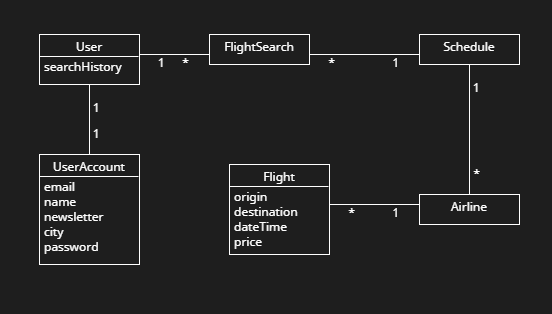
\includegraphics{resources/dataRelations.PNG}

\subsubsection{Data Dictionary}

DR2: Domain level data requirement

Class: User
The user is a Traveller or Travel Agency who has a user account in the product.

Examples:
1. A traveller who has a user account.
2. A travel agency who uses their user account to search flights.

Attributes:
email:      Text, 320 chars
            The user's email address. This email address is used for communication with the user outside the product.

name:       Text, 50 chars
            The name of the traveller or travel agency using the account.

newsletter: Boolean
            Whether the user wants mass email's from the product or not.

city:       Text, 35 chars
            The city the user's default origin is set to. This is the standard origin used when performing searches for the user.

\subsubsection{Virtual window}
Create a virtual window that shows the data that is to be displayed in the system. 

See this example 

\begin{longtable}{|p{3cm}|p{9cm}|}
    \hline
    \rowcolor{headergray}
    \textbf{Field} & \textbf{Value} \\ \hline
    \textbf{Email} & exampleJohn@gmail.com \\ \hline
    \textbf{Name} & John Doe \\ \hline
    \textbf{Utskick} & True \hspace{1em} False \\ \hline
    \textbf{City} & New York \\ \hline
\end{longtable}

\vspace{1cm} % Space between tables

\begin{longtable}{|p{3cm}|p{3cm}|p{3cm}|}
    \hline
    \rowcolor{headergray}
    \textbf{From} & \textbf{Price Max} & \textbf{To} \\ \hline
    NY & 3000 SEK & CPH \\ \hline
    CPH & 2500 SEK & NY \\ \hline
    ... & ... & ... \\ \hline
\end{longtable} % Commented out because it's not relevant in new structure 

% \section{Quality Requirements}
% Simon Persson
% Describe the quality attributes of the system, such as performance, usability, etc.
% \subsection{Quality Requirements}

\renewcommand{\arraystretch}{1.3} % Adjust row height
\definecolor{lightgray}{gray}{0.9} % Define header color

\begin{longtable}{|c|c|p{4.5cm}|p{3.5cm}|p{3.5cm}|}
    \hline
    \rowcolor{lightgray} \textbf{FR ID} & \textbf{QR ID} & \textbf{Description} & \textbf{Measurement} & \textbf{Why} \\
    \hline
    \endfirsthead

    \multicolumn{5}{c}{\textit{(Continued from previous page)}} \\
    \hline
    \rowcolor{lightgray} \textbf{FR ID} & \textbf{QR ID} & \textbf{Description} & \textbf{Measurement} & \textbf{Why} \\
    \hline
    \endhead

    \hline
    \multicolumn{5}{r}{\textit{Continued on next page}} \\
    \endfoot

    \hline
    \endlastfoot

    F1-G & Q1-P & Search results should be displayed within 2 seconds for a standard query. & Tested by generating random inputs and measuring response time using automated performance testing tools, logging response times for 1000+ random queries. & If too slow, users may switch to competitors. \\
    \hline
    F2-D & Q2-D & The system should support flexible date ranges spanning at least 30 days for price comparisons. & Test by selecting a range of 30-60 days, verifying the system returns results across all days without errors. & To be added \\
    \hline
    F3-D & Q3-D & Location detection should be completed in under 3 seconds with at least 95\% accuracy. & Use GPS data from 50 ore more test cases across different devices and measure accuracy based on expected vs. detected locations. & To be added \\
    \hline
    F4-D & Q4-P & The system should retrieve and display flight prices within 2 seconds for a standard query. & Execute automated tests simulating 1000+ searches and log the response time until results are fully rendered. Primarily same as Q1-P & To be added \\
    \hline
    F5-P & Q5-P & The list should support sorting by price, duration, and airline, with sorting applied in under 1 second. & Use UI performance tests to time sorting actions on datasets of varying sizes for example destinations with a lot of flights or destinations with less flights. & To be added \\
    \hline
    F6-P & Q6-P & The system should allow searching for up to 10 passengers simultaneously without affecting response time. & Compare response times of searches with 1 vs. 10 passengers under normal and peak loads. & To be added \\
    \hline
    F7-P & Q7-D & The heatmap should update dynamically within 3 seconds of data input or changes. & Time updates after input changes for example destination, price range or starting point across different devices.  & To be added \\
    \hline
    F8-D & Q8-D & The map should reflect date changes in under 2 seconds without requiring a full reload. & Monitor UI logs to confirm rendering completion time after date modifications. & To be added \\
    \hline
    F9-P & Q9-P & Destination lists should be updated in real-time when new flight deals become available. & Insert a new deal in the back-end or get deal from airlines API and verify update propagation within milliseconds. & To be added \\
    \hline
    F10-P & Q10-P & Clicking a flight should navigate to the booking page within 1 second and fill in relevant details from users account. & Use automated UI testing to time redirection and fill in data according to users account. & To be added \\
    \hline
    F11-P & Q11-P & Selected airports should be highlighted instantly and search results updated in under 2 seconds. & Measure UI update times via browser dev tools or performance logs. & To be added \\
    \hline
    F12-P & Q12-P & The system should retrieve multi-flight prices in less than 5 seconds, considering layovers and airlines. & Run tests for complex multi-leg searches, logging response times for different scenarios. & To be added \\
    \hline
    F13-G & Q13-G & Travel agency accounts should support handling at least 50 concurrent searches without slowdown. & Simulate 50+ concurrent users with load-testing tools for example JMeter and measure system response time. & To be added \\
    \hline
    F14-P & Q14-D & The registration process should take no longer than 15 seconds, including email verification. & Automate user sign-ups and measure time from form submission to receiving the verification email. & To be added \\
    \hline
    F15-D & Q15-D & Email verification links should be sent within 5 seconds and expire after 24 hours. & Log email dispatch times in the system and verify expiration behavior after 24 hours. & To be added \\
    \hline
    F16-P & Q16-P & Changes to email addresses should be confirmed within 10 seconds via a verification email. & Track the end-to-end time from submission of email change request to email receipt. & To be added \\
    \hline
    F17-P & Q17-P & Password changes should be effective after 5 seconds and require strong passwords (at least 8 characters, uppercase, lowercase, number, symbol). & Verify enforcement of password complexity rules and Ensure old credentials become invalid 5 seconds after post-update. & To be added \\
    \hline
    F18-P & Q18-P & Reset emails should be sent within 10 seconds and expire after 30 minutes. & Log email dispatch times and attempt password resets after 30 minutes to confirm expiration. & To be added \\
    \hline
    F19-D & Q19-D & Marketing email preferences should be configurable and updated in real-time. & Toggle marketing settings in the Account management section and verify backend logs reflect changes 5 seconds. & To be added \\
    \hline
    F20-P & Q20-P & Favorite cities should be stored 5 seconds and retrievable in under 1 second. & Save favorite cities and time retrieval speed via API performance monitoring. & To be added \\
    \hline
    F21-G & Q21-G & Reports should be generated in under 10 seconds for a dataset covering the last 6 months. & Execute test report requests and measure query execution and rendering time. & To be added \\
    \hline
    F22-P & Q22-P & Marketing emails should be delivered to 95\% of recipients within 1 minute of sending. & Track email delivery timestamps for mass campaigns and compute success rate over time. & To be added \\
    \hline

\end{longtable}

% usability quality requirements using existing standards
% - && Q23 & - & The ease of use of the product shall be tested and must achieve a System Usability Score (SUS) of at least 70 points, indicating acceptable usability.  \\

% - && Q24 & - & The accessibility of the product shall be tested and must comply with WCAG 2.1 standards.  \\

% Kommentarer för funcational och quality reqs från Övning
% Lägg till Airlines krav att fetcha priser på en vis tid, så vi inkuderar den stakelines.
% Lägg till IT Maintannce krav om att snabbt och säkert kunna använda systemet
% Kolla igenom AND och OR

 % Commented out because it's not relevant in new structure 

\end{document}
